\chapter{Caso Concreto - IoT sensore Temperatura}
%correggere introduzione
Uno degli ambiti in cui viene maggiormente sfruttato Redis é quello IoT.
\paragraph{Cos'é l'IoT?\\}
L''Internet of Things é una tecnologia che permette di massimizzare le capacitá di raccolta e di utilizzo
dei dati da una moltitudine di sorgenti, le quali possono essere prodotti industriali, sistemi di fabbrica, veicoli
di trasporto e cosí via.
L'IoT consente di rendere disponibili i dati che servono a comprendere meglio il mondo reale.
Permette di estrarre informazioni utili ai processi decisionali.\\
Queste informazioni utili devono essere immagazzinate in maniera piú o meno persistente
e devono essere elaborate con dei tempi di latenza piuttosto brevi, ed é proprio qua che interviene Redis.

In questo capitolo verrá analizzata una possibile applicazione in ambito industriale, ma non solo:
verrá utilizzato un sensore di temperatura e umiditá che preleva delle informazioni ad intervalli regolari e
sfrutteremo Redis per la persistenza e l'organizzazione dei dati e l'elaborazione di essi.

\section{Scelte di progetto}
Per questo tipo di applicazione non si necessita di una fase di progettazione, in quanto
nell'ambito che stiamo discutendo abbiamo una mole di dati elevati ma semplici.
Peró, Prima di sviluppare lo sketch vero e proprio dobbiamo decidere che strutture dati messe a disposizione si adattano
maggiormente al nostro caso d'uso.
Possono esserci diversi tipi di implementazione; approfondiamo due modalitá potenzialmente utilizzabili:
una per casi piú semplificati ed una per casi piú avanzati (in cui si potrebbe sfruttare anche una rete di sensori).

Queste modalitá dipendono direttamente dalla struttura dati che intendiamo utilizzare in Redis per salvare i valori;
i due approcci in questione sono:
\begin{enumerate}
    \item metodo semplificato, dove ogni valore prelevato dal sensore lo memorizziamo in Redis con il tipo stringa,
    quindi avremo una tupla che viene generata per ogni prelevamento ad intervalli regolari, e sará cosí composta:\\
    key -> \textbf{nameSensor.time}\\
    value -> \textbf{sensor.value} \\
    Un esempio possibile quindi:\\
    sensorTemp.11:23:49 $\to$ 27.8
    \item metodo avanzato, dove viene utilizza una struttura piú complicata, non presente nelle strutture dati di base di Redis,
    chiamata \texttt{RedisTimeSeries}, é un modulo aggiuntivo che é stato fatto su misura per questo tipo di applicazioni.
    Permette un alto volume di inserimenti di valori con letture a bassa latenza. Puó essere vista come una SortedSet che associa
    ad ogni valore inserito un timestamp come score.\\
    Infatti sará fatto in questo modo:\\
    si crea una serie temporale il cui nome sará quello del sensore e all'interno della serie temporale verranno aggiunti i valori
    prelevati a intervalli temporali, e questi valori verranno associati al timestamp che corrisponde
    al momento in cui vengono inseriti.

    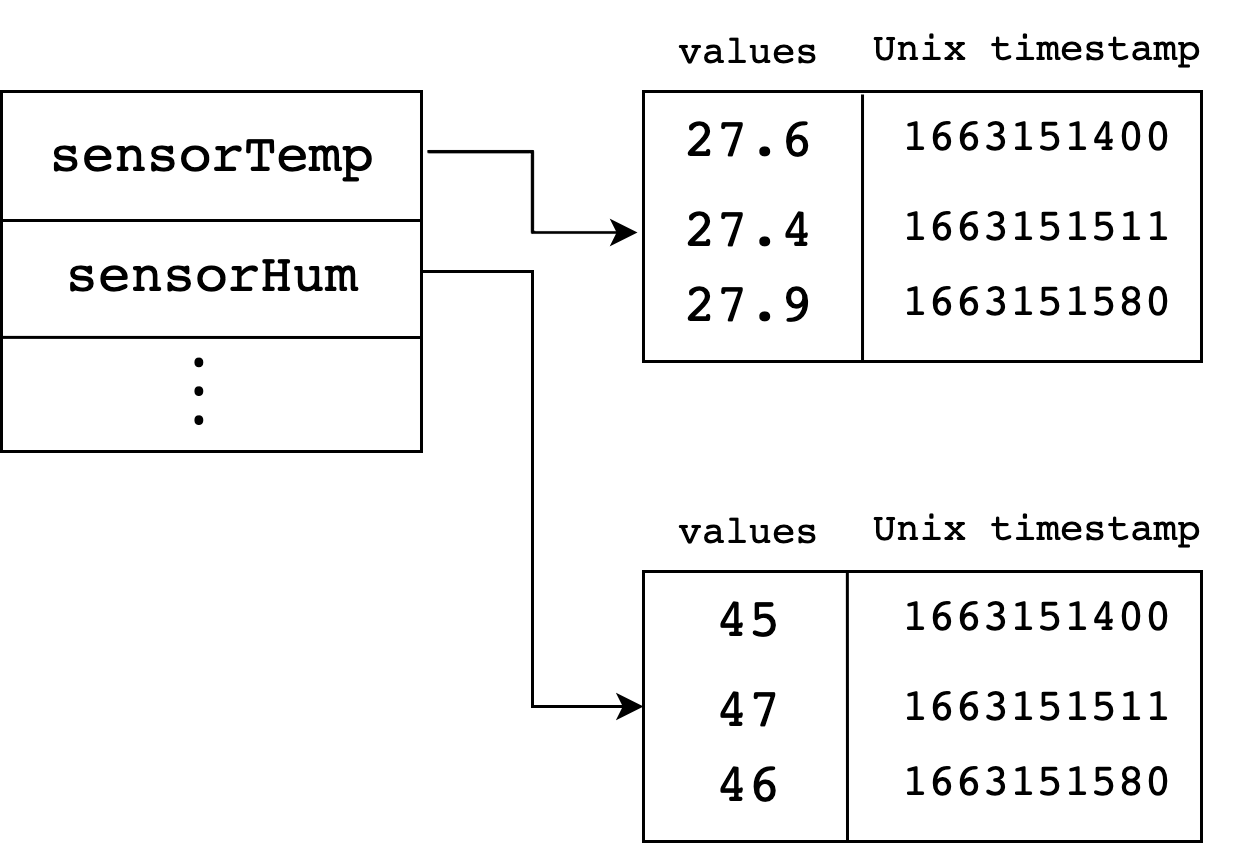
\includegraphics[width=0.7\textwidth]{img/redistimeseries}
\end{enumerate}

\\

Prima dello sviluppo vero e proprio dello sketch necessitiamo di un ultimo passaggio, ovvero apportare dei cambiamenti al file di configurazione del server Redis
Per fare questo vi é una libreria, chiamata \texttt{Redis.h} la quale permette di comunicare con il database Redis.
Eseguiamo una connessione sulla rete Locale sfruttando il modulo WiFi di ESP32.


in quanto con la configurazione standard il server comunica solo su \texttt{localhost}(127.0.0.1).
Dobbiamo aggiungere un parametro per fare in modo che il server sia raggiungibile sulla rete locale aggiungendo indirizzo IP
privato della macchina sulla quale viene eseguito il processo \texttt{redis-server}.
Di conseguenza, il server sará raggiungibile tramite indirizzo IP e Port.\\
Nel nostro caso é: \textbf{192.168.179.25:6379}.
Dobbiamo anche aggiungere una password di sicurezza per l'autenticazione con il server, anche questo viene fatto
aggiungendo un parametro nel file di configurazione.

La configurazione viene modificata cosí:
\begin{lstlisting}[autogobble]
bind  127.0.0.1  192.168.178.25

requirepass "admin"\end{lstlisting}

\\

Per quanto riguarda la persistenza nei file di configurazione, possiamo lasciare quella base, che é una RDB.
Per queste applicazioni non é necessario avere un massimo livello di persistenza.

\section{Arduino e DHT11}
Dopo aver fatto le considerazioni precedenti possiamo passare allo sviluppo dello sketch vero e proprio, che avrá il compito
di inviare dati/informazioni al nostro database.
Il materiale necessario per questo progetto é:
\begin{itemize}
    \item Un microcontrollore compatibile con l'ambiente di sviluppo arduino e, possibilmente, con WiFi integrato,
          nel nostro caso utilizziamo un ESP32.
    \item un sensore digitale di temperatura e umiditá dell'aria, utilizziamo un DHT11: costituito da una parte resistiva
    che si occupa della rilevazione dell'umiditá e da un NTC che rileva la temperatura, queste due parti sono gestite
    da un microcontrollore che é parte integrante del sensore.
\end{itemize}

Dopo che abbiamo collegato il tutto e verificato che il sensore funzioni correttamente, ovvero che mandi dei dati
coerenti all'ESP32 possiamo cominciare a sviluppare il progetto.

\subsection{Connessione con Redis}
Per comunicare ed inviare dati a Redis vi é una libreria apposita, sviluppata proprio per l'ambiente Arduino, chiamata \texttt{Redis.h},
la quale permette di comunicare con il \texttt{redis-server}.\\
Colleghiamoci come client alla rete Locale, grazie al modulo WiFi di ESP32, sfruttando la libreria \texttt{WiFi.h}.\\
Nel metodo di \texttt{setup()}, che é il metodo che viene eseguito solo alla prima esecuzione dello sketch, andiamo a creare una connessione alla rete Locale tramite WiFi e, soprattutto, con il \texttt{server-redis}.
\begin{lstlisting}[autogobble]
#define WIFI_SSID "wifi-name"
#define WIFI_PSW "wifi-psw"
#define REDIS_ADDR "192.168.178.25"
#define REDIS_PORT 6379
#define REDIS_PASSWORD "admin"

WiFiClient RedisConn;
Redis redis(redisConn);

void setup(){
    WiFi.mode(WIFI_STA);  //ESP32 associato come client alla rete WiFi
    WiFi.begin(WIFI_SSID, WIFI_PASSWORD);
    Serial.print("Connecting to the WiFi");
    while (WiFi.status() != WL_CONNECTED)
        delay(250);

    if (!redisConn.connect(REDIS_ADDR, REDIS_PORT))
    {
        Serial.println("Failed to connect to the Redis server!");
        return;
    }

    auto connRet = redis.authenticate(REDIS_PASSWORD);
    if (connRet == RedisSuccess)
    {
        Serial.println("Connected to the Redis server!");
    }
    else
    {
        Serial.printf("Failed to authenticate to the Redis server! Errno: %d\n", (int)connRet);
        return;
    }
}
\end{lstlisting}

Per quanto riguarda la connessione al Server Redis,  con \texttt{redisConn.connect(...)} creiamo una connessione con il server
passando indirizzo Ip e Porta che individuano il processo \texttt{redis-server}, successivamente proviamo ad autenticarci con
\texttt{redis.authenticate(...)}. Se tutto viene eseguito correttamente abbiamo il nostro \texttt{redis-client} che puó
comunicare.


\subsection{NTP}
Come specificato nella sezione dedicata alle scelte progettuali, qualunque modalitá venga utilizzata dobbiamo ricavare l'orario,
indipendentemente che sia uno Unix timestamp o una data in formato hh:mm:ss.
\paragraph{Come facciamo a ricavare l'ora attuale?\\}
Arduino essendo sprovvisto di RTC (Real Time Clock), ovvero un componente elettronco che misura il tempo, ha bisogno di ottenere l'informazione
sull'orario in qualche modo.
Per fare questo sfruttiamo \textbf{NTP} (Network Time Protocol), che é un protocollo client-server utilizzato appunto per allineare orari di applicazioni
e prodotti elettronici.
É disponibile una libreria arduino chiamata \texttt{NTPClient} che permette di collegarsi a un server NTP specificato ed ottenere
l'ora da questo server.

\begin{lstlisting}[autogobble]
const char* ntpServer = "pool.ntp.org";
const long  gmtOffset_sec = 0;
const int   daylightOffset_sec = 7200;

void setup(){
configTime(gmtOffset_sec, daylightOffset_sec, ntpServer);  //configurazione per ottenere orario in formato hh:mm:ss con fuso orario Europeo
}
\end{lstlisting}

Questo é il setup necessario per ottenere l'ora nel formato \texttt{hh:mm:ss}.\\

Invece, se vogliamo ottenere l'orario in Unix Timestamp, la configurazione é la seguente:
\begin{lstlisting}[autogobble]
const char* ntpServer = "pool.ntp.org";

void setup(){
configTime(0, 0, ntpServer);  //configurazione per ottenere orario in Unix Timestamp
}
\end{lstlisting}

\subsection{Invio dataSet}
Adesso possiamo creare la parte di codice che permette di inviare il dataSet a Redis.
Analizziamo i due casi specificati nelle scelte progettuali:
\begin{enumerate}
    \item Il primo tratta la casistica in cui viene adoperata la struttura dati piú semplice, ovvero la stringa:
\begin{lstlisting}[autogobble]
tm getTime(){
  struct tm timeinfo;
  if(!getLocalTime(&timeinfo)){
    Serial.println("Failed to obtain time");
  }
  return timeinfo;
}

void loop(){
 struct tm timeinfo;
 timeinfo = getTime();
 char timeHour[3];
 strftime(timeHour, 3, "%H", &timeinfo);
 char timeMinutes[3];
 strftime(timeMinutes, 3, "%M", &timeinfo);
 char timeSeconds[3];
 strftime(timeSeconds, 3, "%S", &timeinfo);
 sprintf(currentTime, "%s:%s:%s", timeHour, timeMinutes, timeSeconds );

 char valueTemp[10];
 sprintf(valueTemp,"%2.1f",float(dht.readTemperature()));
 char keyTemp[10];
 sprintf(keyTemp,"sensorTemp.%s", currentTime);
 if(redis.set(keyTemp, valueTemp)){
    redis.expire(keyTemp, 600);
 }

 char valueHum[10];
 sprintf(valueHum, "%d", int(dht.readHumidity()));
 char keyHum[10];
 sprintf(keyHum, "sensorHum.%s", currentTime);
 if(redis.set(keyHum, valueHum)){
    redis.expire(keyHum, 600);
  }

 delay(5000);
}\end{lstlisting}

con il metodo \texttt{getTime()} si ottiene l'informazione sull'orario grazie al protocollo NTP.\\
Per quanto riguarda Redis utilizziamo il metodo \texttt{redis.set()} a cui passiamo due parametri:
il primo é la chiave ed il secondo il valore. Ripetiamo il procedimento per la temperatura e l'umiditá.
Con \texttt{redis.expire()} diamo una scadenza alla chiave, la durata della chiave viene
espressa in secondi e viene passata come parametro del metodo.
Alla fine di \texttt{loop()} mettiamo un \texttt{delay()} che indica la pausa che deve intercorrere tra l'esecuzione
di un loop e quello successivo, ovvero dovrá ripetersi ogni 5000 ms (5 secondi).

    \item Di seguito analizziamo la casistica in cui viene adoperata la struttura piú avanzata, RedisTimeSeries:
\begin{lstlisting}[autogobble]
long getTime() {
  time_t now;
  struct tm timeinfo;
  if (!getLocalTime(&timeinfo)) {
    return 0;
  }
  time(&now);
  return now;
}

void loop()
{
   redis.tsadd("sensorTemp", getTime(), dht.readTemperature()*fattoreMoltiplicativoTemp))
   redis.tsadd("sensorHum", getTime(), dht.readHumidity())){
   delay(5000);
}\end{lstlisting}

    Con \texttt{getTime()} otteniamo l'orario in Unix Timestamp, quindi rispetto allo sketch precedente
    sará molto piú semplice l'implementazione, in quanto non dovremo fare conversioni particolari per ottenere
    un formato come quello che dovevamo ottenere nel caso precedente.
    Con il metodo \texttt{redis.tsadd} andiamo ad aggiungere ad una serie temporale un nuovo valore associandolo con il proprio timestamp,
    se la serie temporale non esiste viene creata direttamente con questa istruzione.
    Questo metodo ha un difetto, i valori inseriti possono essere solo interi, quindi, quando andiamo ad inserire
    una nuova temperatura dovremo utilizzare un fattore moltiplicativo pari ai decimali presenti nella sua rilevazione.
    Bisogna ricordarsi di tenerne conto nel software applicativo.
\end{enumerate}


\section{Java}
Per sviluppare il software applicativo viene adoperato Java, lo scopo é quello di generare due grafici differenti,
uno per la temperatura e uno per l'umiditá, sfruttando il dataset presente in Redis ed aggiornandolo in tempo reale, con
una frequenza di aggiornamento pari alla frequenza con cui i dati vengono inviati al server.

\subsection{Jedis e RedisTimeSeries}
Redis mette a disposizione un numero elevato di librerie, per i due approcci vengono utilizzate due librerie differenti,
in quanto la libreria base adoperata nel primo approccio non fornisce metodi necessari per sfruttare la struttura dati piú avanzata
utilizzata nel secondo approccio:
É stato utilizzato:
\begin{enumerate}
    \item il client Jedis, uno dei piú conosciuti. In particolare é stata sfruttata la classe JedisPool per stabilire la connessione
    con \texttt{redis-server}.
 \begin{lstlisting}[autogobble, title={\texttt{RedisClient.java}}]
private static JedisPool jedisPool;

public RedisClient(String ip, int port, int timeout, String password) {
 try {
   if (jedisPool == null) {
    JedisPoolConfig poolConfig = new JedisPoolConfig();
    jedisPool = new JedisPool(poolConfig, ip, port, timeout, password);
   }
 } catch (Exception e) {
            System.out.println("Malformed server address");
   }
}

public Set<String> getKeysByString(String interrogation){
  try (Jedis jedis = jedisPool.getResource()) {
    return jedis.keys(interrogation);
  } catch (Exception ex) {
      System.out.println("Exception caught in KEYS");
    }
  return null;
}

public List<String> getValuesByKeys(Set<String> keys){
 String[] arrayKeys = Utility.convertSetToArray(keys);
 try (Jedis jedis = jedisPool.getResource()) {
  List<String> values = jedis.mget(arrayKeys);
    return values;
 } catch (Exception ex) {
     System.out.println("Exception caught in mget");
   }
 return null;
}
\end{lstlisting}

   Nel costruttore \texttt{RedisClient(...)} creiamo la connessione con il server.\\
   Successivamente, sono stati creati due metodi fondamentali:
    \begin{itemize}
        \item \texttt{getKeysByString(...)}: riusciamo ad ottenere l'insieme chiavi presenti nel database data una certa stringa,
        viene  sfruttato il metodo \texttt{jedis.keys(interrogation)} che ritorna un set di stringhe dato un certo pattern.
        L'idea é quella di ottenere un set composto da tutte le chiavi che cominciano per \texttt{sensorTemp} ed un altro set
        che comincia per \texttt{sensorHum}.
        \item \texttt{getValuesByKeys(...)}: riusciamo ad ottenere l'insieme di valori dato un set di chiavi, questo viene ottenuto grazie
        al metodo \texttt{jedis.mget(arrayKeys)}, che ritorna una lista di valori. Questo metodo vuole come parametro in ingresso
        un array di chiavi, quindi bisogna fare una conversione da set ad array.
    \end{itemize}

    \item il client RedisTimeSeries, creato appositamente per sfruttare la omonima struttura dati.
    \begin{lstlisting}[autogobble, title={\texttt{RedisClient.java}}]
private static final long RANGE_OF_TIME = 600000; //in millisecondi
private RedisTimeSeries client;

public RedisClient(String host, int port, int timeout, int poolSize, String password){
 try {
   client = new RedisTimeSeries(host, port, timeout, poolSize, password);
 }catch (Exception e){
           System.out.println("connection failed!");
 }
}

public Value[] getValues(String key){
 Value[] arrayTemp = client.range(key, System.currentTimeMillis()-RANGE_OF_TIME, System.currentTimeMillis());
 return arrayTemp;
}

public void alterRange(String key){
       client.alter(key, RANGE_OF_TIME, null);
}
\end{lstlisting}
    Nel costruttore \texttt{RedisClient(...)} viene sempre creata la connessione con \texttt{redis-server}.\\
    Analizziamo i due metodi creati:
    \begin{itemize}
        \item \texttt{getValues(...)}:  otteniamo un array di \texttt{Value}, che é una classe messa a disposizione
        dalla libreria \textbf{RedisTimeSeries}, la quale possiede come attributi valore e timestamp.
        Viene sfruttato il metodo \texttt{client.range(...)}, il quale ha il compito di ottenere un insieme di valori associati a timestamp in un certo
        range temporale. Come parametro in ingresso a \texttt{getValues()} dobbiamo fornire una stringa che corrisponde  alla chiave della serie temporale.
        \item \texttt{alterRange(...)}: serve per far scadere valori all'interno di una serie temporale. Viene sfruttato il metodo \texttt{client.alter(...)}.
        Viene fatta la differenza con il timestamp del valore piú recente all'interno della serie; i valori con una differenza maggiore del range specificato vengono eliminati.
        Metodo utilizzato per non far saturare la serie temporale con valori vecchi e poco significativi.
    \end{itemize}
\end{enumerate}



\subsection{DataSet RealTime}
Dopo che abbiamo ottenuto l'intero dataset dal server bisogna modificarlo in modo da renderlo adatto per l'elaborazione grafica.
Per rendere semplice la sua elaborazione in entrambi gli approcci é stata sfruttata una \texttt{TreeMap} che ha le chiavi
di tipo \texttt{LocalTime} ed i valori di tipo \texttt{String}.
Come abbiamo fatto nei due approcci :
\begin{enumerate}
    \item abbiamo dovuto estrarre da ogni elemento del set di chiavi la data, quindi da ogni chiave abbiamo dovuto estrarre la data e convertirla
    in un \texttt{LocalTime}.
    Ad esempio, se abbiamo una chiave fatta in questo modo sensorTemp.12:24:25 estraiamo 12:24:25 e lo convertiamo in tipo \texttt{LocalTime} con l'apposito metodo.
    Dopo di che, associamo ad ogni data il proprio valore e inseriamo tutto in una \texttt{TreeMap} in modo da mantenere l'ordine temporale.
    \item qui invece siamo partiti da un array di tipo \texttt{Value}, e abbiamo dovuto convertire lo Unix timestamp in un \texttt{LocalTime} e successivamente associare date
    e valori nella \texttt{TreeMap} come sopra.
\end{enumerate}
Dopo questo passaggio i due approcci si fondono insieme, in quanto da qui in poi si lavora sulle \texttt{TreeMap} generate che sono esattamente identiche.\\

A questo punto rimane un ultimo problema, ovvero aggiornare il dataset in tempo reale.
Ogni 5 secondi bisogna comunicare con Redis per ottenere i dati aggiornati.

Per fare questo sfruttiamo i Thread.


\begin{lstlisting}[autogobble, title={\texttt{DataSetRealTime.java}}]
private TimeSeries ts = new TimeSeries("f(t)","Time","No:of files");

public void run() {
 while(true) {
   DataSet dataSet = new DataSet(...);
   for(Map.Entry<LocalTime, String> entry : dataSet.getKeyValueMap().entrySet()) {
     LocalTime localTime = entry.getKey();
     double val = Utility.convertStringToDouble(entry.getValue(), div);
     Second istant = new Second(localTime.getSecond(), localTime.getMinute(), localTime.getHour(), LocalDate.now().getDayOfMonth(), LocalDate.now().getMonth().getValue(), LocalDate.now().getYear());
     ts.addOrUpdate(istant, val);
   }
   try {
       Thread.sleep(5000);
   } catch (InterruptedException ex) {
       System.out.println(ex);
   }
 }
}
\end{lstlisting}

In questa classe abbiamo implementato l'interfaccia \texttt{Runnable} e abbiamo fatto un override sul metodo \texttt{run()}.
l'attributo di tipo \texttt{TimeSeries ts} fa parte della libreria \textbf{JFreeChart}, che é stata sfruttata per il disegno dei grafici.
Questa classe funziona in modo analogo ad una Map, peró contiene dei metodi aggiuntivi dedicati alle serie temporali.\\
Con l'istruzione \texttt{new DataSet(...)} andiamo a creare la \texttt{TreeMap} spiegata in precedenza, successivamente
andiamo ad estrarre orario e valore di ogni entry con un ciclo for ed andiamo ad aggiungerlo alla \texttt{TimeSeries} con
il metodo \texttt{ts.addOrUpdate(...)}. Questo metodo aggiunge nuove entry all'interno della sua struttura se vede nuovi istanti,
le lascia inalterate se sono composte da stesso istante e stesso valore associato, mentre le modifica se vede stesso istante e valore associato
modificato.

Tutte queste istruzione vengono ripetute all'infinito grazie a \texttt{while(true)} ed eseguite ad intervalli temporali regolari,
grazie a \texttt{Thread.sleep(5000)}, che ha il compito di disattivare il thread per 5000 ms e dopo riavviarlo.


\subsection{JFreeChart}
Per generare il grafico finale vero e proprio abbiamo sfruttato una libreria adatta alla creazione di diagrammi temporali, che supporta una frequenza di
aggiornamento di questo tipo. Nel caso in cui volessimo sfruttate frequenze di aggiornamento molto piú elevate questa libreria non é adatta,
bisognerebbe utilizzare soluzioni proprietarie, o fatte ad hoc per il caso d'uso in questione.

\begin{lstlisting}[autogobble, title={\texttt{DataSetRealTime.java}}]
DataSetRealTime dataRealTime = new DataSetRealTime(...);
new Thread(dataRealTime).start();

TimeSeriesCollection dataset = new TimeSeriesCollection(dataRealTime.getTimeSeries());
JFreeChart chart = ChartFactory.createTimeSeriesChart(..., dataset, ...);
... //istruzioni grafiche
\end{lstlisting}

Con l'istruzione \texttt{new Thread(dataRealTime).start()} eseguiamo il metodo \texttt{run()}
illustrato in precedenza su un thread specifico.\\
Il grafico vero e proprio viene creato con \texttt{ChartFactory.createTimeSeriesChart()}, a cui
va passato come parametro d'ingresso il dataset e altri parametri per la grafica.


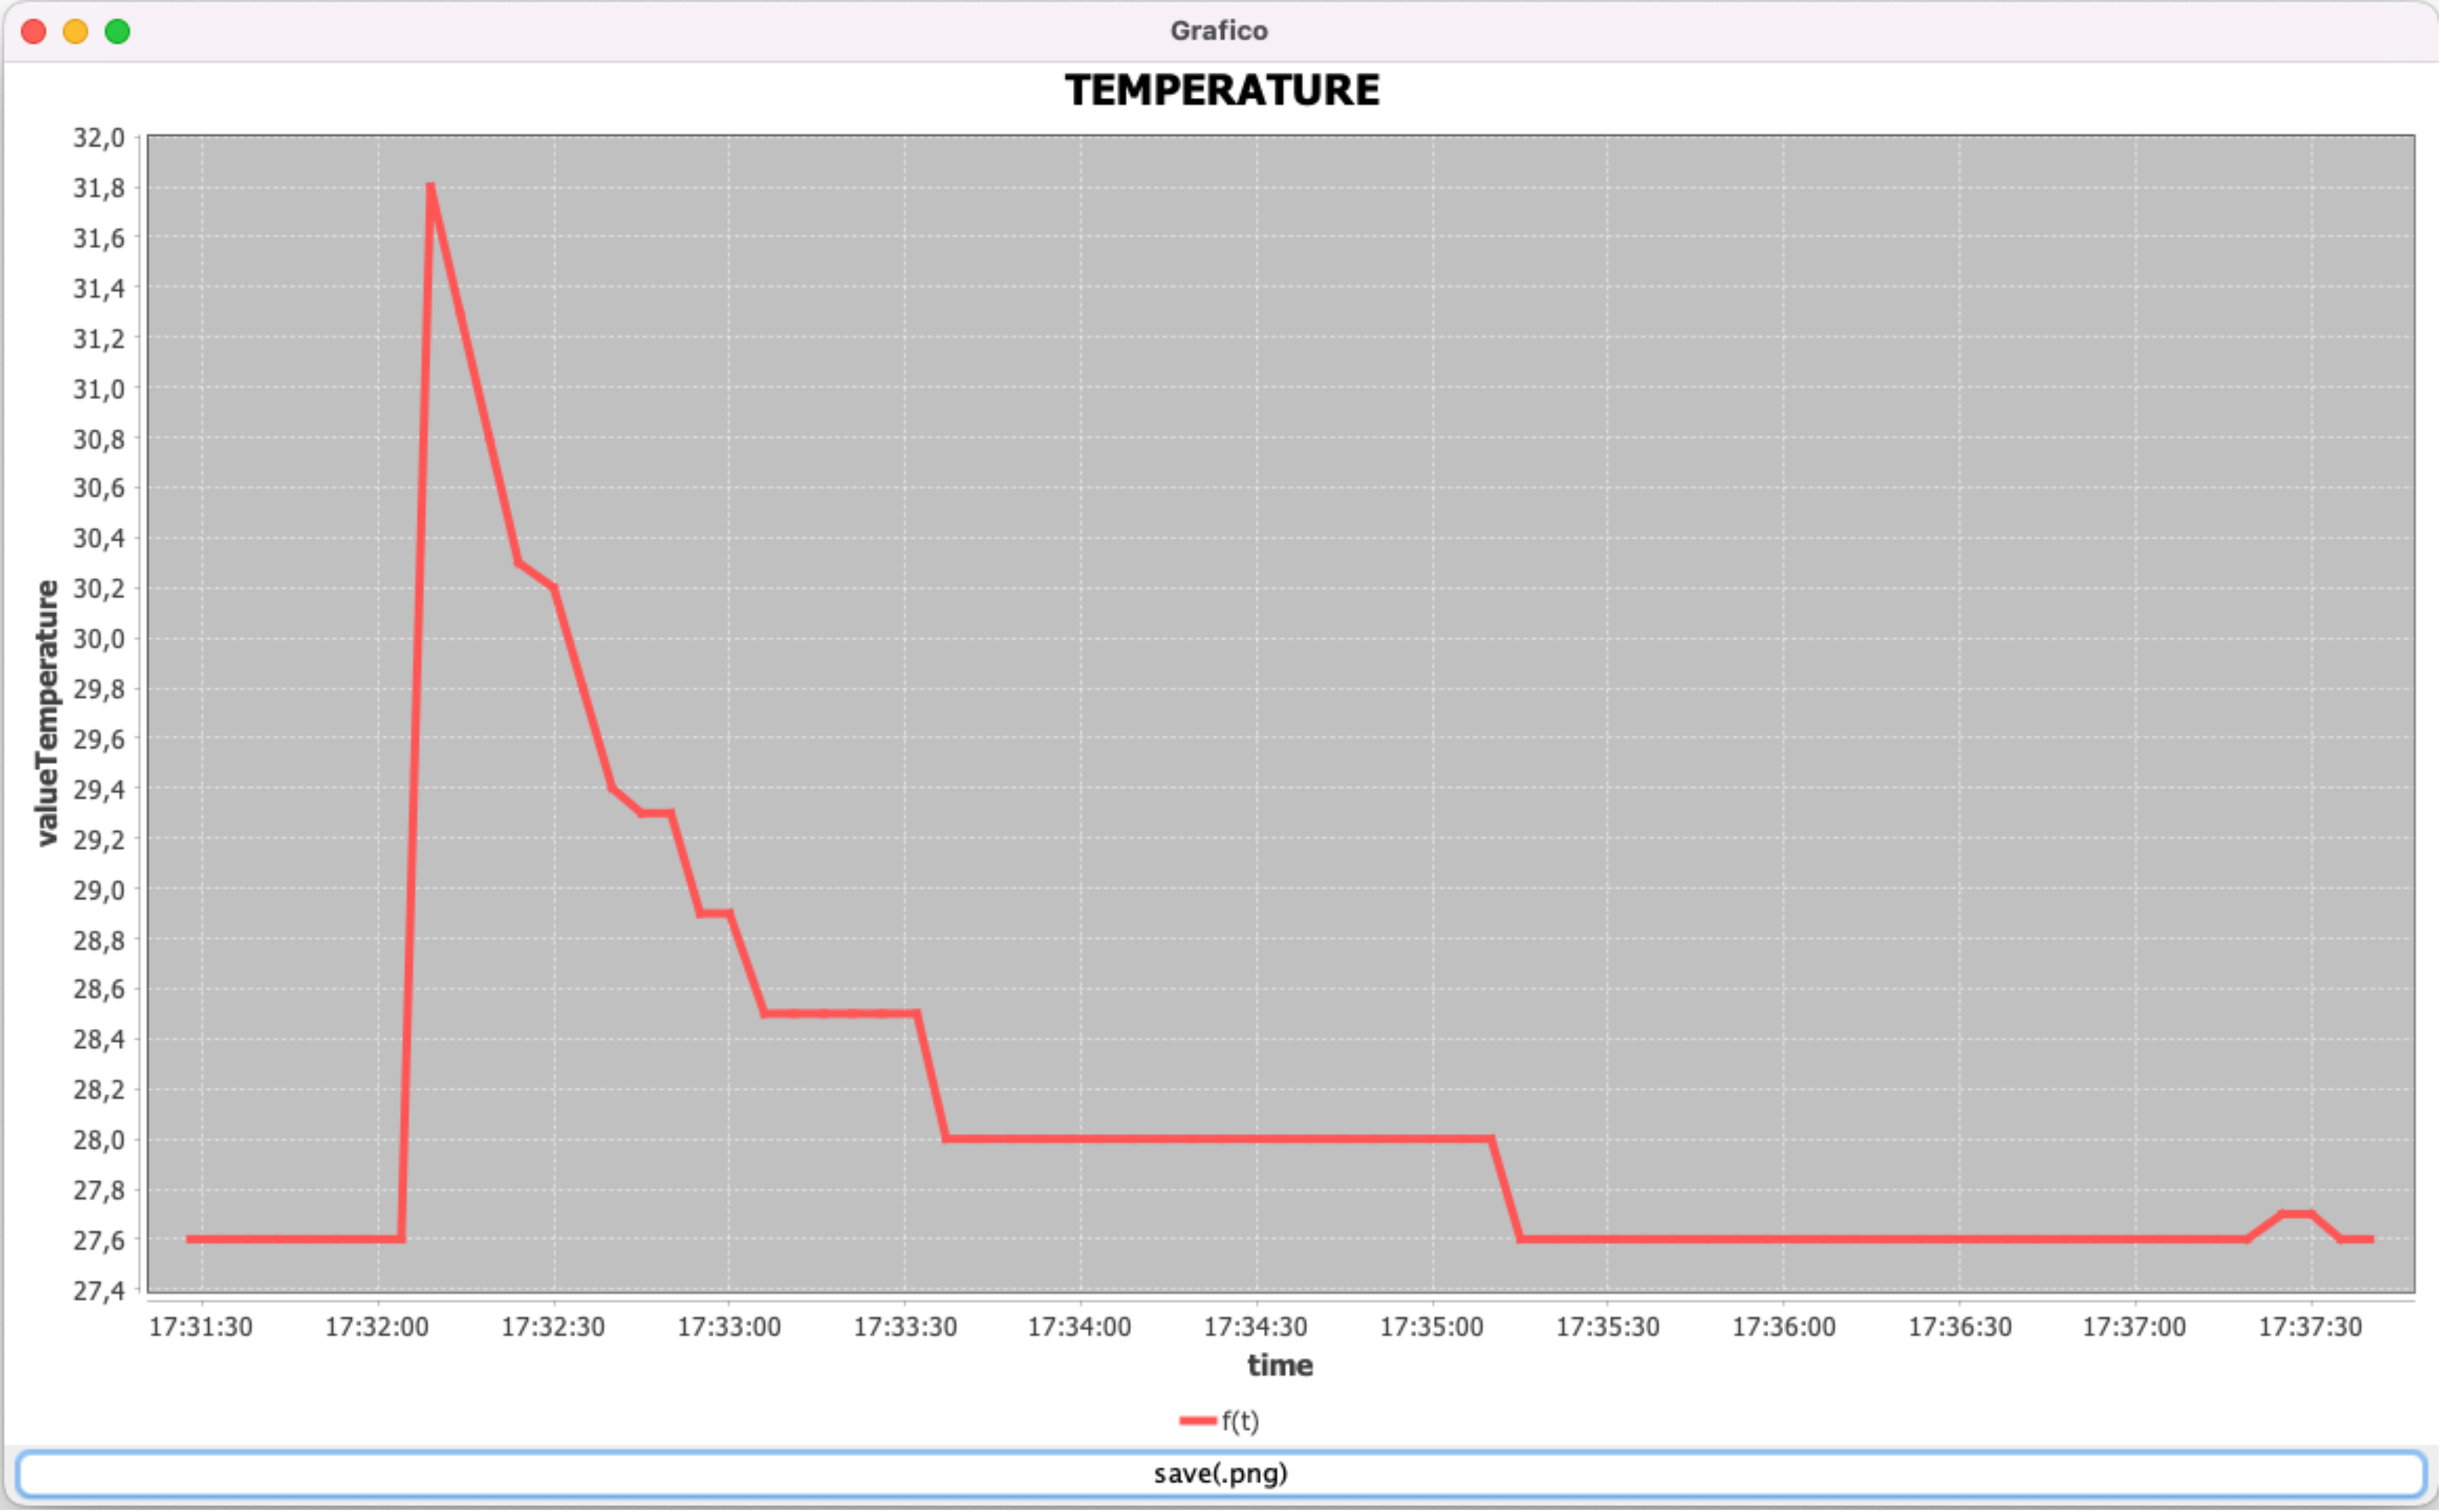
\includegraphics[width=1\textwidth]{img/chartTemperature}
\\


Nell'immagine sopra riportata possiamo apprezzare il risultato finale del progetto.